\documentclass{standalone}
\usepackage{tikz}

\begin{document}

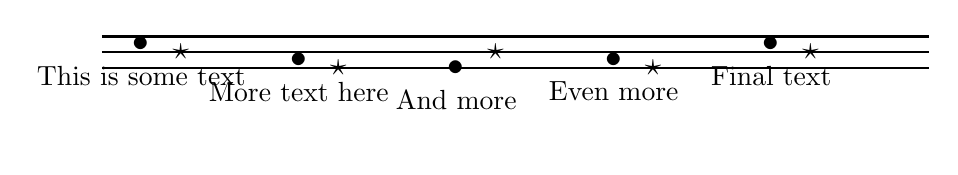
\begin{tikzpicture}[scale=0.5]

% Paper background
\fill[white] (0,0) rectangle (21,3);

% Lines on the paper
\draw[black, thick] (0,2.8) -- (21,2.8); % Top line
\draw[black, thick] (0,2.4) -- (21,2.4); % Middle line
\draw[black, thick] (0,2) -- (21,2); % Bottom line

% Symbols on the paper
\node at (1, 2.6) {\textbf{\large $\bullet$}};
\node at (5, 2.2) {\textbf{\large $\bullet$}};
\node at (9, 2) {\textbf{\large $\bullet$}};
\node at (13, 2.2) {\textbf{\large $\bullet$}};
\node at (17, 2.6) {\textbf{\large $\bullet$}};

% Additional symbols for variety
\node at (2, 2.4) {\textbf{\large $\star$}};
\node at (6, 2) {\textbf{\large $\star$}};
\node at (10, 2.4) {\textbf{\large $\star$}};
\node at (14, 2) {\textbf{\large $\star$}};
\node at (18, 2.4) {\textbf{\large $\star$}};

% Text placeholder
\node at (1, 1.8) {This is some text};
\node at (5, 1.4) {More text here};
\node at (9, 1.2) {And more};
\node at (13, 1.4) {Even more};
\node at (17, 1.8) {Final text};

\end{tikzpicture}

\end{document}